\section{Theoretical Analysis}
\label{sec:analysis}
\subsection{DC components}
First of all, we performed an operating point analysis in order to check if the transistors were operating in the forward active region, both in the gain stage and in the output stage (since the output signal will not have a DC component, there isn't much more purpose to this part of the analysis). For DC analysis, we consider the capacitors to perform as open-circuits (low frequency approximation) - this way, no current flows through the input source and the load, so the DC voltage in both is null. The bias circuit was substituted by its Thévenin equivalent in order to make calculations more simple. The input source is purely sinusoidal, so both $V_{S}$ and $R_{S}$ don't come into play here. For the transistors we used a simplification of the Ebbers-Moll model for forward-active regions. With this, for npn transistors, the voltage drop must occur from the collector to base and from base to emitter - this last voltage drop is approximated with the ideal diode model voltage (0.7V). The current coming out of the emitter must be the sum of the base and collector currents. The same process happens with the pnp transistor, but in a symmetrical fashion. 
In table~\ref{tab:data} we present the DC voltage data for the gain stage, and in table~\ref{tab:data2} we present the equivalent for the output stage
\begin{table}[h!]
  \centering
  \begin{tabular}{|l|r|}
    \hline    
    {\bf Name} & {\bf Values} \\ \hline
    \input{th_data_tab} 
  \end{tabular}
  \caption{Operating point analysis results (gain stage).}
  \label{tab:data}
\end{table}
We assumed the predicted current direction for $I_C$, $I_B$, and $I_E$, and all these currents are positive - so far so good. Since VCE is greater than VBEON, VCB is also positive, which means the voltage drop occurs from the collecter, to the base, to the emitter - the transistor does operate in the forward-active region

\begin{table}[h!]
  \centering
  \begin{tabular}{|l|r|}
    \hline    
    {\bf Name} & {\bf Values} \\ \hline
    \input{outoper_tab} 
  \end{tabular}
  \caption{Operating point analysis results (output stage).}
  \label{tab:data2}
\end{table}
Again the transistor currents are all positive. The collecter is the ground in this case, and since VO2 (which is the same as VEC in this case) is greater than VEBON, VBC is also positive - the voltage drop goes from the emitter all the way to the collector (ground in this case) and this transistor also operates in the forward-active region. We're good to go!

\subsection{Gain Stage}
Now, we move on to analyse the AC components. Recurring to the incremental model for a transistor, we were able to derive equations for the input and output impedances of the gain stage, as well as the voltage gain obtained for the output signal of this stage:

\begin{equation}
  Z_i=R_B||r_{\pi};
\end{equation}

\begin{equation}
  Z_o=R_{C1}||r_o;
\end{equation}

\begin{equation}
  A_V = -g_{m}*Z_{o}*\frac{Z_i}{Z_{i}+R_{S}};
\end{equation}

The constants used, $r_{\pi}$, $r_o$ and $g_m$, are the input resistance, output resistance and transconductance of the incremental transistor model. In table~\ref{tab:gain} we present the results obtained (the negative gain only symbolizes the inversion of the voltage signal direction, and the gain is also calculated solely in relation to the voltage source, without the effect of its resistance):

\begin{table}[h]
  \centering
  \begin{tabular}{|l|r|}
    \hline    
    {\bf Name} & {\bf Values} \\ \hline
    \input{gain_tab} 
  \end{tabular}
  \caption{Gain stage theoretical results.}
  \label{tab:gain}
\end{table}

The input impedance we obtained is considerably larger than $R_S$, which means we will not lose much voltage amplitude in the input part of this stage, which is appropriate. We can clearly see the need for an output stage though, given the magnitude of the output impedance - since it is so much greater than the load resistance, it would consume almost all voltage amplitude, leaving us with a very small voltage amplitude in the load, the exact opposite of our goal. The gain is also significant, and we'll strive for a unitary gain in the output stage in order not to sacrifice this.

\subsection{Output Stage}
Again, using the incremental model, we derived equations for the input and output impedances, and the gain of the output stage of the circuit:

\begin{equation}
  A_V = \frac{g_\pi+g_m}{g_\pi+g_m+g_o+(\frac{1}{R_{E2}})};
\end{equation}

\begin{equation}
  Z_i=\frac{r_\pi}{1-A_V};
\end{equation}

\begin{equation}
  Z_o=\frac{1}{\frac{1}{g_m}||r_\pi||r_o||R_{E2}};
\end{equation}

In table~\ref{tab:output} we present the results obtained:

\begin{table}[h]
  \centering
  \begin{tabular}{|l|r|}
    \hline    
    {\bf Name} & {\bf Values} \\ \hline
    \input{output_tab} 
  \end{tabular}
  \caption{Output stage theoretical results.}
  \label{tab:output}
\end{table}
\pagebreak

As desired, the input impedance of this stage is more than 10 times greater than the output impedance of the gain stage. This is important because the output impedance of the gain stage and the input impedance of the output stage form a voltage divider, and the voltage in the output stage's input impedance is the one that follows through. Having a much greater impedance in this last impedance guarantees then a very small amplitude loss, which allows us to preserve the incoming gain. As well, the output impedance of this stage is desirably low when compared to the 8 Ohm of the speakers resistance, which allows the vast majority of the final gain to flow through the load, thus allowing us to truly have an amplified voltage in our output. The gain for this stage is almost unitary, which means the first stage gain is preserved, as hoped.
At last, the total circuit gain results.

\subsection{Global circuit}
With the same model, we derived similar equations for the circuit as a whole, which will always to directly compare results with the NGSpice simulation (the input impedance is independent from the load, so it will be the same as the input impedance from the gain stage):

\begin{equation}
  Z_o=\frac{1}{\frac{1}{r_{(\pi)2}+Z_{O1}}||g_{o2}||g_{m2}\frac{r_{(\pi)2}}{r_{(\pi)2}+Z_{O1}}||\frac{1}{R_{E2}}};
\end{equation}

\begin{equation}
  A_V=\frac{\frac{1}{r_{(\pi)2}+Z_{O1}}+\frac{g_{m2}r_{(\pi)2}}{r_{(\pi)2}+Z_{O1}}}{\frac{1}{r_{(\pi)2}+Z_{O1}}+\frac{g_{m2}r_{(\pi)2}}{r_{(\pi)2}+Z_{O1}}+\frac{1}{R_{E2}}+\frac{1}{r_{o2}}}A_{V1};
\end{equation}

In table~\ref{tab:outputt} we present the results obtained:

\begin{table}[h]
  \centering
  \begin{tabular}{|l|r|}
    \hline    
    {\bf Name} & {\bf Values} \\ \hline
    \input{circuit_tab} 
  \end{tabular}
  \caption{Total circuit theoretical gain results.}
  \label{tab:outputt}
\end{table}

The gain is slightly lower than the product of the two previous gains, likely due to some signal loss in the interface between stages. The output impedance is now clearly bigger, but still smaller than the load resistance. Even though we experience a greater loss of amplitude, we can still consider this set of data a good result depending on how big the gain is to compensate this increase in the output impedance.

\subsection{Frequency response}
Using the incremental model once again, but this time considering the capacitors' impedances, we ran a frequency response analysis for the gain and the phase difference of the output signal (on the load) in relation to the input signal (voltage source plus its resistance). We did this running a nodal method analysis of the incremental circuit for a vaste branch of frequencies. Figures~\ref{fig:gainfreq} and~\ref{fig:phasefreq} expose the results obtained:

\begin{figure}[!h] \centering
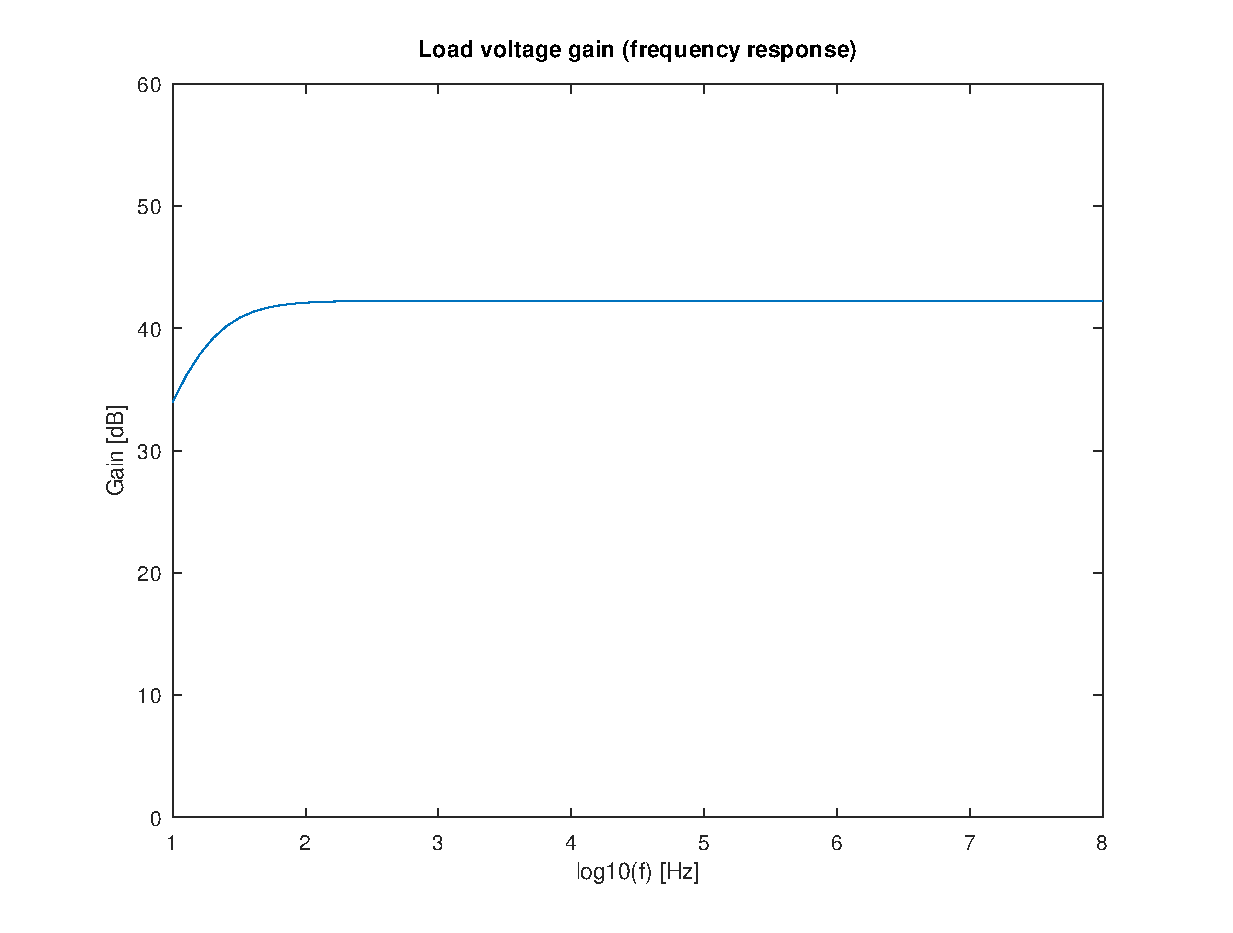
\includegraphics[width=0.6\linewidth]{Gain.eps}
\caption{Load output voltage gain (frequency response).}
\label{fig:gainfreq}
\end{figure}

\begin{figure}[!h] \centering
\includegraphics[width=0.6\linewidth]{Phase.eps}
\caption{Load output voltage phase difference (frequency response).}
\label{fig:phasefreq}
\end{figure}

\pagebreak

Looking to the gain plot, we would be hoping to achieve the likes of a band-pass filter (as it will be obtained in simulation). However, we only achieved a high-pass filter. This is due to the fact that we didn't consider the capacitors of the transistors themselves, which would cause the gain to fall for high frequencies. With our plot, the gain stabilizes for medium frequencies, and keeps its momentum for high frequencies - the upper cut-off frequency is then something always tending to infinity with this model. We did manage to measure the lower cut-off frequency and a more accurate measure of gain for each frequency (since we considered the capacitors in this analyse). Regarding the phase plot, we notice that the phase difference stabilizes in the 180º degrees for medium frequencies, thus confirming the inversion of the signal voltage direction in the output. In table~\ref{tab:freq} we present the results:

\begin{table}[h]
  \centering
  \begin{tabular}{|l|r|}
    \hline    
    {\bf Name} & {\bf Values} \\ \hline
    \input{frequency_tab} 
  \end{tabular}
  \caption{Gain for medium frequencies and lower cut-off frequency of the output voltage signal.}
  \label{tab:freq}
\end{table}

The lower cut-off frequency yielded close to 20 Hz, the lowest frequency the human ear can perceive as a musical note, and the lower limit pretended for this amplifier - this is a very suitable result. This was achieved by finding the point on the gain frequency response plot that had a 3 decibel drop relative to the maximum gain.
